%%%%%%%%%%%%%%%%%%%%%%%%%%%%%%%%%%%%%%%%%%%%%%%%%%%%%%%%%%%%%%%%%%%%%%%%%%%%%%%%%%
% Demo: a ReAct weather agent built by hand in LangGraph.
% Order: problem, design, then one code piece per slide, assemble, visualise, run, summary.
\begin{frame}[fragile]\frametitle{}
\begin{center}
{\Large Agent Demo: ReAct from Scratch (Weather)}

{\tiny (Ref: LangGraph documentation, docs.langchain.com)}
\end{center}
\end{frame}

%%%%%%%%%%%%%%%%%%%%%%%%%%%%%%%%%%%%%%%%%%%%%%%%%%%%%%%%%%%
\begin{frame}[fragile]\frametitle{What is a ReAct Agent?}
      \begin{itemize}
        \item \textbf{ReAct} = Reasoning + Acting (Yao et al., 2022, arXiv 2210.03629).
        \item \textbf{Loop}: Think \(\rightarrow\) Act (tool call) \(\rightarrow\) Observe (tool result) \(\rightarrow\) Think \(\dots\)
        \item The LLM reasons about the goal, calls a tool, reads the result, and repeats until it can answer.
        \item It mirrors flexible, human-like problem solving, not a fixed workflow.
        \item In LangGraph the whole loop is a shared \textbf{state object} updated by two nodes.
        \item A prebuilt version exists (\texttt{create\_agent}); we build a simple one by hand to see every part.
      \end{itemize}
\end{frame}

%%%%%%%%%%%%%%%%%%%%%%%%%%%%%%%%%%%%%%%%%%%%%%%%%%%%%%%%%%%
\begin{frame}[fragile]\frametitle{The Problem: A Weather Agent}
      \begin{itemize}
        \item \textbf{Question} from a user: "What is the weather in Berlin on 2026-10-27?"
        \item A language model alone cannot answer: it has no live data, and it may invent a forecast.
        \item It needs to \textbf{ask a weather service} and then \textbf{explain the result} in plain words.
        \item So the agent must: (1) notice that data is needed, (2) call a weather tool with a city and a date, (3) read the tool result, (4) write the answer.
        \item Sometimes one tool call is not enough (two cities), so the agent must be able to \textbf{loop}.
        \item This is exactly the ReAct loop: the model decides, the tool acts, the model reads the result.
      \end{itemize}
\end{frame}

%%%%%%%%%%%%%%%%%%%%%%%%%%%%%%%%%%%%%%%%%%%%%%%%%%%%%%%%%%%
\begin{frame}[fragile]\frametitle{The Design: Two Nodes and One Decision}
\adjustbox{valign=t}{%
\begin{minipage}{0.52\linewidth}
      \begin{itemize}
        \item \textbf{State}: the messages so far plus a step counter; it flows through every node.
        \item \textbf{Node} \texttt{llm}: the chat model reads the messages and either answers or asks for a tool.
        \item \textbf{Router} \texttt{should\_continue}: reads the last message. Tool calls present? Go to \texttt{tools}. Otherwise END.
        \item \textbf{Node} \texttt{tools}: runs the requested tool and adds its result as a message.
        \item \textbf{Normal edge} \texttt{tools} \(\rightarrow\) \texttt{llm}: closes the loop.
      \end{itemize}
\end{minipage}%
}%
\hfill%
\adjustbox{valign=t}{%
\begin{minipage}{0.44\linewidth}
\begin{center}
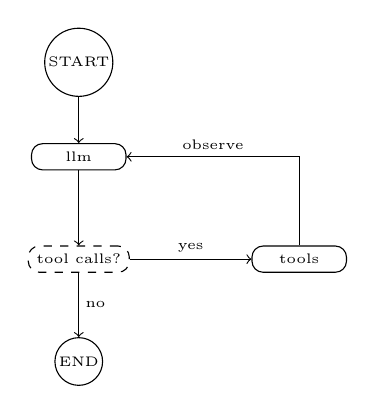
\begin{tikzpicture}
\tiny
\node[draw,circle,inner sep=1pt] (s) at (0,3.4) {START};
\node[draw,rounded corners,minimum width=1.2cm,inner sep=3pt] (l) at (0,2.2) {llm};
\node[draw,dashed,rounded corners,inner sep=3pt] (r) at (0,0.9) {tool calls?};
\node[draw,circle,inner sep=1pt] (e) at (0,-0.4) {END};
\node[draw,rounded corners,minimum width=1.2cm,inner sep=3pt] (t) at (2.8,0.9) {tools};
\draw[->] (s) -- (l);
\draw[->] (l) -- (r);
\draw[->] (r) -- node[right] {no} (e);
\draw[->] (r) -- node[above] {yes} (t);
\draw[->] (t) |- node[near end,above] {observe} (l);
\end{tikzpicture}
\end{center}
\tiny{The dashed box is the conditional edge: one decision, two possible next steps.}
\end{minipage}%
}
\end{frame}

%%%%%%%%%%%%%%%%%%%%%%%%%%%%%%%%%%%%%%%%%%%%%%%%%%%%%%%%%%%
\begin{frame}[fragile]\frametitle{Setup}
      \begin{itemize}
        \item Default model: a small one on your own computer, so no API key and no per-token charge.
        \item In LM Studio, download a small model that supports tool calling (for example \texttt{qwen3-1.7b}) and start the local server (Developer tab).
        \item One file, \texttt{llm\_config.py}, holds the model name for every example.
      \end{itemize}
\begin{lstlisting}[language=Python]
conda env create -f environment.yml     # Code/langgraph: LangGraph 1.x, LangChain 1.x
conda activate langgraph

python llm_config.py      # prints the model ids the server offers
# put that id in MODEL_NAME, or:  LLM_MODEL=<id>   (PowerShell: $env:LLM_MODEL = "<id>")
# cloud back ends only: put the API key in the environment, never in code
\end{lstlisting}
\end{frame}

%%%%%%%%%%%%%%%%%%%%%%%%%%%%%%%%%%%%%%%%%%%%%%%%%%%%%%%%%%%
\begin{frame}[fragile]\frametitle{Step 1: Define the State}
      \begin{itemize}
        % [upgrade-deck: commented out 2026-10-19 | Task 2 | repeats the Core Concepts slides; shortened to a recap]
        % \item The state is the \textbf{context object} that flows through every node. You declare its fields; a \texttt{TypedDict}, a dataclass or a Pydantic class all work (Pydantic adds validation and defaults).
        % \item A \textbf{reducer} says how an update is merged. With none, a new value \textbf{overwrites} the old one; \texttt{add\_messages} \textbf{appends} to the list instead.
        % \item The counter shows that state can hold more than messages; we use it as a step limit.
        % \item \texttt{MessagesState} is only a ready-made state with a \texttt{messages} field; using it is optional.
        \item Recap: the state is the context object every node reads and updates; a Pydantic class is one way to declare it.
        \item \texttt{messages} uses the \texttt{add\_messages} reducer, so replies are \textbf{appended}, not overwritten.
        \item \texttt{number\_of\_steps} is our own field: the step limit for the router.
      \end{itemize}
\begin{lstlisting}[language=Python]
from typing import Annotated
from langchain_core.messages import AnyMessage
from langgraph.graph.message import add_messages
from pydantic import BaseModel, Field

class AgentState(BaseModel):
    messages: Annotated[list[AnyMessage], add_messages] = Field(default_factory=list)
    number_of_steps: int = 0
\end{lstlisting}
\end{frame}

%%%%%%%%%%%%%%%%%%%%%%%%%%%%%%%%%%%%%%%%%%%%%%%%%%%%%%%%%%%
\begin{frame}[fragile]\frametitle{Step 2: Define the Tool}
      \begin{itemize}
        \item A tool is a plain Python function plus a \textbf{name, description and typed arguments}.
        \item The model reads the description and the argument types to decide when and how to call it.
        \item The helpers \texttt{geocode} and \texttt{fetch\_hourly} (city to coordinates, then Open-Meteo) are in \texttt{react\_agent.py}.
      \end{itemize}
\begin{lstlisting}[language=Python]
from langchain_core.tools import tool

@tool
def get_weather_forecast(location: str, date: str) -> str:
    """Get min, max and mean temperature (deg C) for a city on a date (yyyy-mm-dd)."""
    coords = geocode(location)                      # city -> (lat, lon)
    temps = fetch_hourly(*coords, date)             # Open-Meteo: hourly temperatures
    return json.dumps({"min_c": min(temps), "max_c": max(temps),
                       "mean_c": sum(temps) / len(temps)})

tools = [get_weather_forecast]
\end{lstlisting}
\end{frame}

%%%%%%%%%%%%%%%%%%%%%%%%%%%%%%%%%%%%%%%%%%%%%%%%%%%%%%%%%%%
\begin{frame}[fragile]\frametitle{Step 3: Choose the Model and Bind the Tool}
      \begin{itemize}
        \item "LLM" and "chat model" are the same object here; we call it \texttt{llm}. \texttt{get\_llm()} reads the one shared config.
        \item \texttt{bind\_tools} only \textbf{advertises} the tools: their name, description and argument types are sent with every request.
        \item The model never runs a tool. It replies with a \texttt{tool\_calls} request, and our \texttt{tools} node runs it.
        \item Always test this step on its own: not every small model calls tools.
      \end{itemize}
\begin{lstlisting}[language=Python]
from llm_config import get_llm

llm = get_llm()                          # the chat model
llm_with_tools = llm.bind_tools(tools)   # the same model, now aware of the tool

reply = llm_with_tools.invoke("What is the weather in Berlin on 2026-10-15?")
print(reply.tool_calls)
# [{'name': 'get_weather_forecast', 'args': {'location': 'Berlin', 'date': '2026-10-15'}, 'id': '...'}]
\end{lstlisting}
\end{frame}

%%%%%%%%%%%%%%%%%%%%%%%%%%%%%%%%%%%%%%%%%%%%%%%%%%%%%%%%%%%
\begin{frame}[fragile]\frametitle{Step 4: The llm Node}
      \begin{itemize}
        \item A node is just a Python function: it reads the state and returns \textbf{only what changed}. Inside it can be anything: an LLM call, an API call, plain code, even a whole agent.
        \item This one sends all messages to the model and adds the reply (an answer or a tool request).
        \item It also adds 1 to the step counter.
      \end{itemize}
\begin{lstlisting}[language=Python]
def call_llm(state: AgentState):
    reply = llm_with_tools.invoke(state.messages)
    return {"messages": [reply],
            "number_of_steps": state.number_of_steps + 1}
\end{lstlisting}
\end{frame}

%%%%%%%%%%%%%%%%%%%%%%%%%%%%%%%%%%%%%%%%%%%%%%%%%%%%%%%%%%%
\begin{frame}[fragile]\frametitle{Step 5: The tools Node}
      \begin{itemize}
        \item Take the tool request from the last AI message and run the tool with its arguments.
        \item Wrap the output in a \texttt{ToolMessage}; \texttt{tool\_call\_id} links the result to the request.
        % [upgrade-deck: commented out 2026-10-19 | Task 5 | "later slide" pointer breaks a standalone slide]
        % \item With several tools, look the tool up by name; the prebuilt \texttt{ToolNode} (later slide) does this for you.
        \item With several tools, look the tool up by name; the prebuilt \texttt{ToolNode} does this for you.
      \end{itemize}
\begin{lstlisting}[language=Python]
from langchain_core.messages import ToolMessage

def call_tools(state: AgentState):
    last = state.messages[-1]                    # the AI message with tool_calls
    results = []
    for call in last.tool_calls:
        output = get_weather_forecast.invoke(call["args"])
        results.append(ToolMessage(content=output, tool_call_id=call["id"]))
    return {"messages": results}
\end{lstlisting}
\end{frame}

%%%%%%%%%%%%%%%%%%%%%%%%%%%%%%%%%%%%%%%%%%%%%%%%%%%%%%%%%%%
\begin{frame}[fragile]\frametitle{Step 6: The Router (Conditional Edge)}
      \begin{itemize}
        \item The router is not a node that changes state; it only \textbf{chooses the next step}.
        \item It returns a label; the label is mapped to a node when we assemble the graph.
        \item The run ends when there is no tool request (a final answer) or the step limit is reached.
      \end{itemize}
\begin{lstlisting}[language=Python]
MAX_STEPS = 6

def should_continue(state: AgentState):
    if state.number_of_steps >= MAX_STEPS:
        return "end"                          # safety: never loop forever
    if not state.messages[-1].tool_calls:
        return "end"                          # no tool wanted: final answer
    return "continue"                         # tool wanted: go run it
\end{lstlisting}
\end{frame}

%%%%%%%%%%%%%%%%%%%%%%%%%%%%%%%%%%%%%%%%%%%%%%%%%%%%%%%%%%%
\begin{frame}[fragile]\frametitle{Step 7: Assemble the Graph}
      \begin{itemize}
        \item Register the nodes, then the edges. Names here match the design picture: \texttt{llm}, \texttt{tools}.
        \item \texttt{compile()} checks the wiring and returns a runnable graph.
      \end{itemize}
\begin{lstlisting}[language=Python]
from langgraph.graph import StateGraph, START, END

workflow = StateGraph(AgentState)
workflow.add_node("llm", call_llm)
workflow.add_node("tools", call_tools)

workflow.add_edge(START, "llm")                  # first node to run
workflow.add_conditional_edges(
    "llm", should_continue,
    {"continue": "tools", "end": END})           # label -> next node
workflow.add_edge("tools", "llm")                # loop back

graph = workflow.compile()
\end{lstlisting}
\end{frame}

%%%%%%%%%%%%%%%%%%%%%%%%%%%%%%%%%%%%%%%%%%%%%%%%%%%%%%%%%%%
\begin{frame}[fragile]\frametitle{Visualise the Compiled Graph}
\adjustbox{valign=t}{%
\begin{minipage}{0.52\linewidth}
      \begin{itemize}
        \item Always draw the graph and compare it with your design.
        \item Solid arrow: normal edge. Dashed arrow: conditional edge, labelled with the router's return value.
        \item In a notebook, the picture appears below the cell. The PNG is drawn by an online service; \texttt{draw\_mermaid()} gives the same graph as text, offline.
      \end{itemize}
\begin{lstlisting}[language=Python]
from IPython.display import Image, display

display(Image(
    graph.get_graph().draw_mermaid_png()))
# offline: print(graph.get_graph().draw_mermaid())
\end{lstlisting}
\end{minipage}%
}%
\hfill%
\adjustbox{valign=t}{%
\begin{minipage}{0.42\linewidth}
\begin{center}
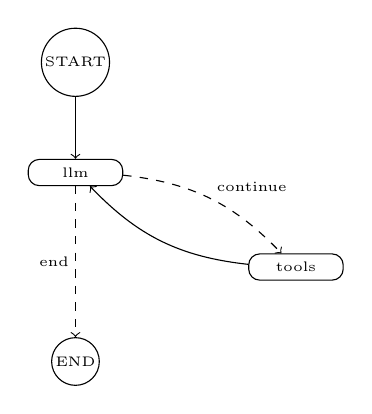
\begin{tikzpicture}
\tiny
\node[draw,circle,inner sep=1pt] (s) at (0,3.4) {START};
\node[draw,rounded corners,minimum width=1.2cm,inner sep=3pt] (l) at (0,2.0) {llm};
\node[draw,circle,inner sep=1pt] (e) at (0,-0.4) {END};
\node[draw,rounded corners,minimum width=1.2cm,inner sep=3pt] (t) at (2.8,0.8) {tools};
\draw[->] (s) -- (l);
\draw[->,dashed] (l) -- node[left] {end} (e);
\draw[->,dashed,bend left=20] (l) to node[above right] {continue} (t);
\draw[->,bend left=20] (t) to (l);
\end{tikzpicture}
\end{center}
\tiny{Output of the compiled graph (redrawn).}
\end{minipage}%
}
\end{frame}

%%%%%%%%%%%%%%%%%%%%%%%%%%%%%%%%%%%%%%%%%%%%%%%%%%%%%%%%%%%
\begin{frame}[fragile]\frametitle{Run the Agent and Stream the Steps}
      \begin{itemize}
        \item \texttt{stream\_mode="values"} yields the full state after every node, so each Think, Act and Observe step is visible.
      \end{itemize}
\begin{lstlisting}[language=Python]
from datetime import datetime

inputs = {"messages": [("user",
          f"What is the weather in Berlin on {datetime.today().date()}?")],
          "number_of_steps": 0}

for state in graph.stream(inputs, stream_mode="values"):
    state["messages"][-1].pretty_print()

# Human Message   -> the question
# Ai Message      -> tool call: get_weather_forecast(Berlin, date)
# Tool Message    -> {"min_c": ..., "max_c": ..., "mean_c": ...}
# Ai Message      -> natural-language answer
\end{lstlisting}
\end{frame}

%%%%%%%%%%%%%%%%%%%%%%%%%%%%%%%%%%%%%%%%%%%%%%%%%%%%%%%%%%%
\begin{frame}[fragile]\frametitle{A Run, Read Top to Bottom}
      \begin{itemize}
        \item The numbers come from a real Open-Meteo call; the layout is simplified. Each streamed state adds one message.
        \item Two LLM calls and one tool call: \texttt{number\_of\_steps} ends at 2.
      \end{itemize}
\begin{lstlisting}
Human Message : What is the weather in Berlin on 2026-10-27?

Ai Message    : (tool call) get_weather_forecast(location="Berlin", date="2026-10-27")

Tool Message  : {"min_c": 12.9, "max_c": 18.6, "mean_c": 15.7}

Ai Message    : The weather in Berlin on 2026-10-27 will be around 15.7 degrees
                Celsius, with a minimum of 12.9 and a maximum of 18.6.
\end{lstlisting}
\end{frame}

%%%%%%%%%%%%%%%%%%%%%%%%%%%%%%%%%%%%%%%%%%%%%%%%%%%%%%%%%%%
\begin{frame}[fragile]\frametitle{State After Each Step, and the Decision}
\begin{itemize}
\item The same run, seen as state. Each node returns only what changed; the state grows by one message.
\item The router reads the last message and picks the next edge.
\end{itemize}
\begin{center}
\small
\adjustbox{max width=\linewidth}{%
\begin{tabular}{p{0.13\linewidth}p{0.42\linewidth}p{0.08\linewidth}p{0.28\linewidth}}
\hline
After node & Messages in the state & Steps & Router decision \\
\hline
START & question & 0 & go to llm \\
llm & question, tool call & 1 & tool call: tools \\
tools & question, tool call, tool result & 1 & back to llm \\
llm & question, tool call, tool result, answer & 2 & no tool call: end \\
\hline
\end{tabular}}
\end{center}
\begin{itemize}
\item The loop stops for one of two reasons: no tool call, or the step limit.
\end{itemize}
\end{frame}

%%%%%%%%%%%%%%%%%%%%%%%%%%%%%%%%%%%%%%%%%%%%%%%%%%%%%%%%%%%
\begin{frame}[fragile]\frametitle{Prebuilt ToolNode and tools\_condition}
      \begin{itemize}
        \item The hand-written \texttt{call\_tools} and \texttt{should\_continue} are so common that LangGraph ships them.
        \item \texttt{ToolNode} runs the tool calls; \texttt{tools\_condition} routes to \texttt{tools} or END.
      \end{itemize}
\begin{lstlisting}[language=Python]
from langgraph.graph import START
from langgraph.prebuilt import ToolNode, tools_condition

workflow = StateGraph(AgentState)
workflow.add_node("llm", call_llm)
workflow.add_node("tools", ToolNode(tools))
workflow.add_edge(START, "llm")
workflow.add_conditional_edges("llm", tools_condition)  # tools or END
workflow.add_edge("tools", "llm")
graph = workflow.compile()
\end{lstlisting}
\end{frame}

%%%%%%%%%%%%%%%%%%%%%%%%%%%%%%%%%%%%%%%%%%%%%%%%%%%%%%%%%%%
\begin{frame}[fragile]\frametitle{One-Line Agent with create\_agent}
      \begin{itemize}
        \item \texttt{create\_agent} (LangChain 1.x, built on LangGraph) builds the whole loop; it replaces \texttt{create\_react\_agent}.
        \item By hand you saw what it does: a model node, a tool node and a router over a shared state.
      \end{itemize}
\begin{lstlisting}[language=Python]
from langchain.agents import create_agent

agent = create_agent(
    model=get_llm(),
    tools=[get_weather_forecast],
    system_prompt="You are a concise weather assistant.",
)
result = agent.invoke(
    {"messages": [("user", "Weather in Berlin on 2026-10-15?")]})
print(result["messages"][-1].content)
\end{lstlisting}
\end{frame}

%%%%%%%%%%%%%%%%%%%%%%%%%%%%%%%%%%%%%%%%%%%%%%%%%%%%%%%%%%%
\begin{frame}[fragile]\frametitle{One Config, Any Model}
      \begin{itemize}
        \item Only the model line is provider-specific; state, nodes and edges stay the same.
        \item Change \texttt{MODEL\_NAME} in \texttt{llm\_config.py}, or set an environment variable, and every example follows.
      \end{itemize}
\begin{lstlisting}[language=Python]
# llm_config.py (shortened)
PROVIDER   = os.getenv("LLM_PROVIDER", "lmstudio")   # lmstudio | ollama | groq
MODEL_NAME = os.getenv("LLM_MODEL") or DEFAULT_MODELS[PROVIDER]
#   lmstudio -> a small local model   (free, no key)
#   groq     -> "openai/gpt-oss-20b"  (needs GROQ_API_KEY)

def get_llm(provider=None, temperature=None, model=None): ...

graph = build_graph(get_llm())                  # the model comes from the config
# LLM_PROVIDER=groq python react_agent.py       # same graph, another back end
\end{lstlisting}
\end{frame}

%%%%%%%%%%%%%%%%%%%%%%%%%%%%%%%%%%%%%%%%%%%%%%%%%%%%%%%%%%%
% [upgrade-deck: moved 2026-10-19 | Task 3 | Demo Summary now follows the extra-features slides; see the merged frame below them]
% \begin{frame}[fragile]\frametitle{Demo Summary}
%       \begin{itemize}
%         \item \textbf{Problem}: answer a weather question with live data, so the model must call a tool.
%         \item \textbf{Design}: two nodes (\texttt{llm}, \texttt{tools}), one router, one loop-back edge.
%         \item \textbf{Code}: state, tool, bound model, three small functions, then \texttt{StateGraph} wires them.
%         \item \textbf{Run}: each streamed state adds one message; the router ends the run on no tool request or the step limit.
%         \item \textbf{Shortcuts}: \texttt{ToolNode} and \texttt{tools\_condition}, or \texttt{create\_agent} for the whole loop.
%       \end{itemize}
% \end{frame}

%%%%%%%%%%%%%%%%%%%%%%%%%%%%%%%%%%%%%%%%%%%%%%%%%%%%%%%%%%%
% [upgrade-deck: renamed 2026-10-19 | Task 3 | title repeated the deck subject; was "Beyond the Basics: What Else LangGraph Offers"]
\begin{frame}[fragile]\frametitle{Beyond the Basics: More Features}
      \begin{itemize}
        \item \textbf{Human in the loop}: \texttt{interrupt()} pauses a node and waits; \texttt{Command(resume=...)} continues. Use it for approval before a payment, a send or a delete, or for editing a draft.
        \item \textbf{Checkpointing and memory}: a checkpointer saves the state after each step; a \texttt{thread\_id} picks the conversation. It enables pause and resume, follow-up questions and replay.
        % [upgrade-deck: commented out 2026-10-19 | Task 5 | "next slide" pointer breaks a standalone slide]
        % \item \textbf{Streaming}: watch progress instead of waiting for the end (next slide).
        \item \textbf{Streaming}: watch progress instead of waiting for the end.
        \item \textbf{Command and Send}: one return value can update state and choose the next node; \texttt{Send} fans out the same node over many items in parallel.
        \item \textbf{Subgraphs and multi-agent}: a node can itself be a graph, so agents can be composed.
        \item Each of these is added to the same graph; the nodes and edges you wrote stay as they are.
      \end{itemize}
\end{frame}

%%%%%%%%%%%%%%%%%%%%%%%%%%%%%%%%%%%%%%%%%%%%%%%%%%%%%%%%%%%
\begin{frame}[fragile]\frametitle{Streaming and Human Approval in a Few Lines}
      \begin{itemize}
        \item \textbf{Stream modes}: \texttt{values} (full state after each step), \texttt{updates} (only what each node changed), \texttt{messages} (LLM tokens as they arrive), \texttt{custom} (your own progress events).
        \item \textbf{Approval}: the graph needs a checkpointer and a \texttt{thread\_id}, so it can stop and come back.
      \end{itemize}
\begin{lstlisting}[language=Python]
for chunk in graph.stream(inputs, stream_mode="updates"):
    print(chunk)                                  # {node_name: what it returned}

from langgraph.types import interrupt, Command
from langgraph.checkpoint.memory import InMemorySaver

def approval(state):                              # a node that waits for a person
    ok = interrupt({"question": "Send this email?"})
    return {"approved": ok}

graph = workflow.compile(checkpointer=InMemorySaver())
cfg = {"configurable": {"thread_id": "t1"}}
graph.invoke(inputs, cfg)                         # runs until interrupt(), then pauses
graph.invoke(Command(resume=True), cfg)           # resumes; ok == True
\end{lstlisting}
\end{frame}

%%%%%%%%%%%%%%%%%%%%%%%%%%%%%%%%%%%%%%%%%%%%%%%%%%%%%%%%%%%
\begin{frame}[fragile]\frametitle{Demo Summary}
      \begin{itemize}
        \item \textbf{Problem}: answer a weather question with live data, so the model must call a tool.
        \item \textbf{Design}: two nodes (\texttt{llm}, \texttt{tools}), one router, one loop-back edge.
        \item \textbf{Code}: state, tool, bound LLM, three small functions; \texttt{StateGraph} wires them.
        \item \textbf{Run}: each streamed state adds one message; the router ends the run on no tool call or the step limit.
        \item \textbf{Shortcuts}: \texttt{ToolNode} and \texttt{tools\_condition}, or \texttt{create\_agent} for the whole loop.
        \item \textbf{Remember}: a node is any Python function, an edge is normal or conditional, the state is the shared context, and the LLM is swappable through one config.
      \end{itemize}
\end{frame}

%%%%%%%%%%%%%%%%%%%%%%%%%%%%%%%%%%%%%%%%%%%%%%%%%%%%%%%%%%%
% [Optional cut 2026-10-19 | LangGraph trim, move to the advanced part | restore by uncommenting this block]
% \begin{frame}[fragile]\frametitle{Continuing the Conversation}
%       \begin{itemize}
%         \item The final state already holds the whole history, so a follow-up just appends a message.
%         \item The agent can re-use earlier results, call the tool again, or compare cities.
%         \item For memory that survives restarts, compile with a checkpointer and pass a \texttt{thread\_id}.
%       \end{itemize}
% \begin{lstlisting}[language=Python]
% state["messages"].append(("user", "Would it be warmer in Munich?"))
%
% for state in graph.stream(state, stream_mode="values"):
%     state["messages"][-1].pretty_print()
% \end{lstlisting}
% \end{frame}

%%%%%%%%%%%%%%%%%%%%%%%%%%%%%%%%%%%%%%%%%%%%%%%%%%%%%%%%%%%
% [Optional cut 2026-10-19 | LangGraph trim, move to the advanced part | restore by uncommenting this block]
% \begin{frame}[fragile]\frametitle{Guardrails for Tools and Steps}
%       \begin{itemize}
%         \item \textbf{Tools never raise into the graph}: return an error string so the model can explain or retry.
%         \item \textbf{Step limit}: the counter in the state stops runaway Think, Act loops.
%         \item \textbf{Validated state}: a wrong type fails at the node boundary, not three steps later.
%       \end{itemize}
% \begin{lstlisting}[language=Python]
% try:
%     coords = geocode(location)
%     ...
% except Exception as exc:               # network, rate limit, bad date
%     return json.dumps({"error": str(exc)})
%
% def should_continue(state: AgentState):
%     if state.number_of_steps >= MAX_STEPS:   # e.g. 6
%         return "end"
%     ...
% \end{lstlisting}
% \end{frame}

%%%%%%%%%%%%%%%%%%%%%%%%%%%%%%%%%%%%%%%%%%%%%%%%%%%%%%%%%%%
% [Optional cut 2026-10-19 | LangGraph trim, move to the advanced part | restore by uncommenting this block]
% \begin{frame}[fragile]\frametitle{Extending the ReAct Agent}
%       \begin{itemize}
%         \item \textbf{More tools}: search, calculator, database; the model picks which to call.
%         \item \textbf{Structured output node}: force the final answer into a Pydantic schema.
%         \item \textbf{Reflection node}: critique the draft answer before returning it.
%         \item \textbf{Memory}: add a checkpointer so threads resume across sessions.
%         \item \textbf{Human approval}: pause before risky tools with \texttt{interrupt}.
%         \item \textbf{Guardrails}: step limits, tool timeouts, retries on transient errors.
%       \end{itemize}
% \end{frame}

%%%%%%%%%%%%%%%%%%%%%%%%%%%%%%%%%%%%%%%%%%%%%%%%%%%%%%%%%%%
% [Optional cut 2026-10-19 | frugal tail removed after the early Frugal AI slide | restore by uncommenting this block]
% \begin{frame}[fragile]\frametitle{Frugal AI: Same Graph, Smaller Model}
%       \begin{itemize}
%         \item The graph did not change when the model went from a cloud API to a file on your laptop. Only the model line did.
%         \item What you gain: no per-token charge, no key, the data stays on the machine, and it works offline.
%         \item What you check: does the small model call the tool, follow the format and stay in the step limit? Test it on your task before you trust it.
%         \item \textbf{Measured} (FrugalAI harness, LM Studio, Q4\_K\_M, 15 runs): \texttt{gemma-2-2b-it} decodes at a median of 10.9 tokens per second with the GPU off (12.2 with a small 2 GB GPU helping), with an engine memory peak of about 3.4 GB. That is a 10-core development PC, not a frugal-tier device.
%         \item Observed: a system message was accepted and followed in LM Studio (one test); but the model ignored the tool schema (0 of 5).
%         \item A fixed workflow with a small model is the frugal default; a free-roaming agent needs a stronger model.
%       \end{itemize}
% \end{frame}

%%%%%%%%%%%%%%%%%%%%%%%%%%%%%%%%%%%%%%%%%%%%%%%%%%%%%%%%%%%
% [Optional cut 2026-10-19 | actual runs not shown in the seminar | restore by uncommenting this block]
% \begin{frame}[fragile]\frametitle{A Small Model and Tools: What Happened}
%       \begin{itemize}
%         \item Real runs: live Open-Meteo data, temperature 0, 5 runs each. Successes out of 5:
%       \end{itemize}
% \begin{center}
% \adjustbox{max width=\linewidth}{%
% \begin{tabular}{lcc}
% \textbf{Method} & \textbf{One city} & \textbf{Two cities} \\
% \hline
% gemma-2-2b-it, \texttt{bind\_tools} agent & 0 (no tool call) & 0 (no tool call) \\
% gemma-2-2b-it, text ReAct agent & 5 & 0 (said Munich) \\
% gemma-2-2b-it, fixed workflow, code compares & - & 5 \\
% qwen3-1.7b, \texttt{bind\_tools} agent & 5 & 5 \\
% \end{tabular}}
% \end{center}
%       \begin{itemize}
%         \item Two cities (Berlin 15.7 C, Munich 12.3 C): the text agent made both calls, then answered "Munich will be warmer".
%         \item Asked to compare two given numbers, gemma was wrong in 5 of 5 tries. When code compared and gemma wrote the sentence, the verdict was right 5 of 5, but it dropped the number until the prompt gave one example.
%         \item qwen3-1.7b (with \texttt{/no\_think}) called the tool and compared correctly; a different small model can behave very differently.
%       \end{itemize}
% \end{frame}

%%%%%%%%%%%%%%%%%%%%%%%%%%%%%%%%%%%%%%%%%%%%%%%%%%%%%%%%%%%
% [Optional cut 2026-10-19 | out of order in the demo; code in Code/langgraph/react_demo/text_react_agent.py | restore by uncommenting this block]
% \begin{frame}[fragile]\frametitle{Text ReAct: Tools Without Tool Calling}
%       \begin{itemize}
%         \item No \texttt{bind\_tools}: a prompt teaches \texttt{Action:}, \texttt{Action Input:} and \texttt{Final Answer:}; the graph parses the text.
%         \item Rules a 2B model needs: an Action beats a Final Answer in the same reply; cut the reply at \texttt{Observation:}; errors come back as Observation text; a step limit.
%         \item It works for one tool call, and it still failed the two-city question. Parsing fixes format, not judgment.
%       \end{itemize}
% \begin{lstlisting}[language=Python]
% # text_react_agent.py (shortened)
% def parse_reply(text):
%     text = re.split(r"\n\s*Observation\s*:", text, maxsplit=1)[0]
%     act = _ACTION.search(text)
%     if act:                       # an Action wins over a Final Answer
%         return "action", act.group(1), raw_input(text, act)
%     fin = _FINAL.search(text)
%     return ("final", fin.group(1).strip(), "") if fin else ("none", text, "")
%
% # call_tool: bad JSON or unknown tool -> an "Observation: {error ...}" message
% # should_continue: pending Action and number_of_steps < max_steps -> "tools"
% \end{lstlisting}
% \end{frame}

%%%%%%%%%%%%%%%%%%%%%%%%%%%%%%%%%%%%%%%%%%%%%%%%%%%%%%%%%%%
% [Optional cut 2026-10-19 | frugal tail removed after the early Frugal AI slide | restore by uncommenting this block]
% \begin{frame}[fragile]\frametitle{Code Decides, the Model Talks}
%       \begin{itemize}
%         \item A fixed workflow: fetch A, fetch B, compare in code, phrase with the model. No loop, no tool calling.
%         \item Code does what must be right: fetch, compare, route, validate. The model does language.
%         \item The answer is checked for the computed numbers; if they are missing, a template sentence is used.
%         \item Live result: "Berlin is 3.4 C warmer than Munich, with a mean of 15.7 C compared to 12.3 C." (5 of 5 identical).
%       \end{itemize}
% \begin{lstlisting}[language=Python]
% # START -> fetch_a -> fetch_b -> compare -> phrase -> END
% def phrase(state):
%     reply = model.invoke(PHRASE_PROMPT.format(facts=state["facts"],
%                                               diff=state["diff_c"]))
%     text = reply.content.strip()
%     if answer_ok(text, state):         # names the warmer city and the "3.4"
%         return {"answer": text, "used_fallback": False}
%     return {"answer": state["facts"], "used_fallback": True}
% \end{lstlisting}
% \end{frame}

%%%%%%%%%%%%%%%%%%%%%%%%%%%%%%%%%%%%%%%%%%%%%%%%%%%%%%%%%%%
% [Optional cut 2026-10-19 | frugal tail removed after the early Frugal AI slide | restore by uncommenting this block]
% \begin{frame}[fragile]\frametitle{Where to Go Next: FrugalAI}
%       \begin{itemize}
%         \item \textbf{FrugalAI repository}: measured benchmarks and recipes for small models on old laptops and Raspberry Pi, with a small harness to measure your own device (tokens per second, memory).
%         \item \textbf{Awesome list}: a curated list of frugal AI efforts by platform (old laptop, Raspberry Pi, phone, microcontroller, browser). Entries must be free to use, use a downloadable model, charge no per-token fee, and say what they were run on.
%         \item \textbf{Contribute}: run something frugal? Add it to the list, or add one measurement from your own device.
%         \item Students and educators are welcome to join.
%       \end{itemize}
% \end{frame}

%%%%%%%%%%%%%%%%%%%%%%%%%%%%%%%%%%%%%%%%%%%%%%%%%%%%%%%%%%%
% [upgrade-deck: commented out 2026-10-19 | Task 2 | duplicates Demo Summary; its points are merged into that frame]
% \begin{frame}[fragile]\frametitle{Takeaways}
%       \begin{itemize}
%         \item \textbf{State is the context object}: one Pydantic model flows through every node.
%         \item \textbf{Nodes are plain functions}: read the state, return only what changed.
%         \item \textbf{Edges decide}: one conditional edge turns a chain into a Think, Act, Observe loop.
%         \item \textbf{The model is swappable}: a small local model or a cloud API, same graph, one config.
%         \item \textbf{Build it once, then use the prebuilt}: \texttt{ToolNode} or \texttt{create\_agent}.
%       \end{itemize}
% \end{frame}

%%%%%%%%%%%%%%%%%%%%%%%%%%%%%%%%%%%%%%%%%%%%%%%%%%%%%%%%%%%
\begin{frame}[fragile]\frametitle{Quick Check: The ReAct Loop}
\begin{block}{Think About It}
In the hand-written ReAct graph, what makes the loop stop and return an answer?
\begin{enumerate}
  \item[A.] The \texttt{tools} node returns END after one call
  \item[B.] The router finds no tool calls in the last AI message (or the step limit is hit)
  \item[C.] The LLM must output the word FINISH
  \item[D.] The graph always stops after two LLM calls
\end{enumerate}
\end{block}
\end{frame}

%%%%%%%%%%%%%%%%%%%%%%%%%%%%%%%%%%%%%%%%%%%%%%%%%%%%%%%%%%%
\begin{frame}[fragile]\frametitle{Quick Check: The ReAct Loop}
\begin{block}{Answer}
\textbf{Correct: B.} \texttt{should\_continue} ends the run when the model replies without tool calls, or when \texttt{number\_of\_steps} reaches the limit. Option A is wrong because \texttt{tools} always loops back to \texttt{llm}; options C and D describe rules that do not exist in this graph.
\end{block}
\end{frame}

%%%%%%%%%%%%%%%%%%%%%%%%%%%%%%%%%%%%%%%%%%%%%%%%%%%%%%%%%%%
% [Archive 2026-10-19 | demo rewrite: problem, design, one code piece per slide | originals of the replaced frames, restore by uncommenting a block]
% \begin{frame}[fragile]\frametitle{The Agent as a Graph}
% \adjustbox{valign=t}{%
% \begin{minipage}{0.56\linewidth}
%       \begin{itemize}
%         \item \textbf{State}: the Pydantic context object (messages and a step counter) that flows through every node.
%         \item \textbf{Node} \texttt{llm}: calls the chat model, which answers or asks for a tool.
%         \item \textbf{Node} \texttt{tools}: runs the requested tool calls and returns \texttt{ToolMessage}s.
%         \item \textbf{Conditional edge}: tool calls present \(\rightarrow\) \texttt{tools}, otherwise \(\rightarrow\) END.
%         \item \textbf{Normal edge}: \texttt{tools} \(\rightarrow\) \texttt{llm}, closing the loop.
%         \item Add more nodes (structured output, reflection) as needed.
%       \end{itemize}
% \end{minipage}%
% }%
% \hfill%
% \adjustbox{valign=t}{%
% \begin{minipage}{0.4\linewidth}
% \begin{center}
% \begin{tikzpicture}
% \tiny
% \node[draw,circle,inner sep=1pt] (s) at (0,3.2) {START};
% \node[draw,rounded corners,minimum width=1.1cm] (l) at (0,1.8) {llm};
% \node[draw,rounded corners,minimum width=1.1cm] (t) at (3,1.8) {tools};
% \node[draw,circle,inner sep=1pt] (e) at (0,0.2) {END};
% \draw[->] (s) -- (l);
% \draw[->,bend left=25] (l) to node[above] {tool calls} (t);
% \draw[->,bend left=25] (t) to node[below] {observe} (l);
% \draw[->] (l) -- node[right] {answer} (e);
% \end{tikzpicture}
% \end{center}
% \tiny{The ReAct loop: the llm node and the tools node alternate until there are no tool calls.}
% \end{minipage}%
% }
% \end{frame}

% [Archive 2026-10-19 | demo rewrite | original Define the Tool]
% \begin{frame}[fragile]\frametitle{Define the Tool}
% \begin{lstlisting}[language=Python]
% # geocode() and fetch_hourly() are small helpers: see react_agent.py
% import json
% from langchain_core.tools import tool
% from pydantic import BaseModel, Field
%
% class SearchInput(BaseModel):
%     location: str = Field(description="The city, e.g., San Francisco")
%     date: str = Field(description="The forecasting date, yyyy-mm-dd")
%
% @tool("get_weather_forecast", args_schema=SearchInput)
% def get_weather_forecast(location: str, date: str) -> str:
%     """Retrieves the weather using the Open-Meteo API.
%     Takes a city and a date (yyyy-mm-dd), returns JSON with min/max/mean."""
%     coords = geocode(location)              # geopy Nominatim
%     if coords is None:
%         return json.dumps({"error": "Location not found"})
%     hourly = fetch_hourly(*coords, date)    # requests.get(open-meteo)
%     ...
%     return json.dumps({"min_c": min(t), "max_c": max(t), "mean_c": avg})
%
% tools = [get_weather_forecast]
% \end{lstlisting}
% \end{frame}

% [Archive 2026-10-19 | demo rewrite | original Choose the Model and Bind the Tool]
% \begin{frame}[fragile]\frametitle{Choose the Model and Bind the Tool}
%       \begin{itemize}
%         \item \texttt{get\_llm()} reads the one shared config, so no example hard-codes a model name.
%         \item \texttt{bind\_tools} sends the tool schema (name, description, argument types) with every request.
%         \item A model that supports tools replies with \texttt{tool\_calls} instead of text. Always test this step first.
%         \item \textbf{Measured}: with \texttt{gemma-2-2b-it} the tool was called in 0 of 5 tries; it answered in plain text ("I can't provide you with a specific weather forecast"). Its model card does not promise tool calling.
%         \item So this graph, as written, does not work with this model. Two fixes follow: text ReAct, or a fixed workflow.
%       \end{itemize}
% \begin{lstlisting}[language=Python]
% from llm_config import get_llm      # MODEL_NAME lives in llm_config.py
%
% llm = get_llm()                     # default: small model in LM Studio
% model = llm.bind_tools(tools)
%
% res = model.invoke("What is the weather in Berlin on 2026-10-15?")
% print(res.tool_calls)
% # [{'name': 'get_weather_forecast', 'args': {...}, 'id': '...'}]
% # gemma-2-2b-it: []   (0 of 5 tries): it answered in text instead
% \end{lstlisting}
% \end{frame}

% [Archive 2026-10-19 | demo rewrite | original The Tool Node and The Model Node and the Routing Edge]
% \begin{frame}[fragile]\frametitle{The Tool Node}
%       \begin{itemize}
%         \item Run every tool call in the last AI message and wrap each result in a \texttt{ToolMessage}.
%         \item \texttt{tool\_call\_id} links the result back to the request.
%         \item The prebuilt \texttt{ToolNode} does exactly this.
%       \end{itemize}
% \begin{lstlisting}[language=Python]
% from langchain_core.messages import ToolMessage
%
% tools_by_name = {t.name: t for t in tools}
%
% def call_tool(state: AgentState):
%     outputs = []
%     for tool_call in state.messages[-1].tool_calls:
%         result = tools_by_name[tool_call["name"]].invoke(tool_call["args"])
%         outputs.append(ToolMessage(content=result,
%                                    name=tool_call["name"],
%                                    tool_call_id=tool_call["id"]))
%     return {"messages": outputs}
% \end{lstlisting}
% \end{frame}
% \begin{frame}[fragile]\frametitle{The Model Node and the Routing Edge}
%       \begin{itemize}
%         \item Each node reads the state (\texttt{state.messages}) and returns only what changed.
%         \item The router ends the run when there is no tool call or when the step limit is hit.
%       \end{itemize}
% \begin{lstlisting}[language=Python]
% def call_model(state: AgentState):
%     response = model.invoke(state.messages)
%     return {"messages": [response],
%             "number_of_steps": state.number_of_steps + 1}
%
% def should_continue(state: AgentState):
%     if state.number_of_steps >= MAX_STEPS:
%         return "end"                       # cycle limit
%     if not state.messages[-1].tool_calls:
%         return "end"                       # final answer reached
%     return "continue"
% \end{lstlisting}
% \end{frame}

% [Archive 2026-10-19 | demo rewrite | original A Real ReAct Trace (text ReAct format, gemma-2-2b-it)]
% \begin{frame}[fragile]\frametitle{A Real ReAct Trace}
%       \begin{itemize}
%         \item A real run of the text ReAct agent with \texttt{gemma-2-2b-it}, live Open-Meteo data. Each streamed state adds one message; read it top to bottom.
%         \item Two LLM calls and one tool call: \texttt{number\_of\_steps} ends at 2.
%       \end{itemize}
% \begin{lstlisting}
% Human Message : What is the weather in Berlin on 2026-10-27?
%
% Ai Message    : Action: get_weather_forecast
%                 Action Input: {"location": "Berlin", "date": "2026-10-27"}
%
% Human Message : Observation: {"location": "Berlin", "date": "2026-10-27",
%                 "min_c": 12.9, "max_c": 18.6, "mean_c": 15.7}
%
% Ai Message    : Final Answer: The weather in Berlin on 2026-10-27 will be
%                 around 15.7 degrees Celsius with a minimum of 12.9 and a
%                 maximum of 18.6 degrees Celsius.
% \end{lstlisting}
% \end{frame}
